\section{Component-based development}
\begin{itemize}
	\item An intermediate language CDL - Component-based Description Language is proposed for programmers
	\item CDL is generated from model or can be created by programmers
	\item CDL is used for whole system implementation, not just architecture description
	\item CDL adds more constructs to OO languages:
	\begin{itemize}
		\item UML State Machine constructs: state, transition, event, pseudo state, action
		
		\item Component constructs: component, part, port, connector
		
		\item Reuse maximally existing constructs in OO languages such as class, attribute
	\end{itemize}
	
	\item CDL is synchronized with models
\end{itemize}

\begin{table}[]
	\centering
	\caption{Mapping between UML and CDL concepts}
	\label{my-label}
	\begin{tabular}{|l|l|l|l|}
		\hline
		UML                                                                  & DCL                                                                 & OO                                                                            & C++                                                            \\ \hline
		\begin{tabular}[c]{@{}l@{}}Class/\\ component\end{tabular}           & Class                                                               & Class                                                                         & Class                                                          \\ \hline
		Part                                                                 & Part                                                                & \begin{tabular}[c]{@{}l@{}}Composition \\ attribute\end{tabular}              & Attribute                                                      \\ \hline
		\begin{tabular}[c]{@{}l@{}}Port \\ (data/control)\end{tabular}       & Port                                                                & Attribute                                                                     & \begin{tabular}[c]{@{}l@{}}Reference \\ Attribute\end{tabular} \\ \hline
		Many ports                                                           & Multiple-port                                                       & \begin{tabular}[c]{@{}l@{}}Multiple\\   interface \\ realization\end{tabular} & --                                                             \\ \hline
		Connector                                                            & \begin{tabular}[c]{@{}l@{}}Binding \\ (static+runtime)\end{tabular} & --                                                                            & Methods                                                        \\ \hline
		State machine                                                        & State machine                                                       & \begin{tabular}[c]{@{}l@{}}Set of classes\\  and methods\end{tabular}         & --                                                             \\ \hline
		\begin{tabular}[c]{@{}l@{}}Provided port \\ constraints\end{tabular} &                                                                     &                                                                               &                                                                \\ \hline
		Interface                                                            & Class/Interface                                                     & Interface                                                                     & Class                                                          \\ \hline
		Signal                                                               & Class                                                               & Class                                                                         & Class/Struct                                                   \\ \hline
	\end{tabular}
\end{table}



\begin{figure}
	\centering
	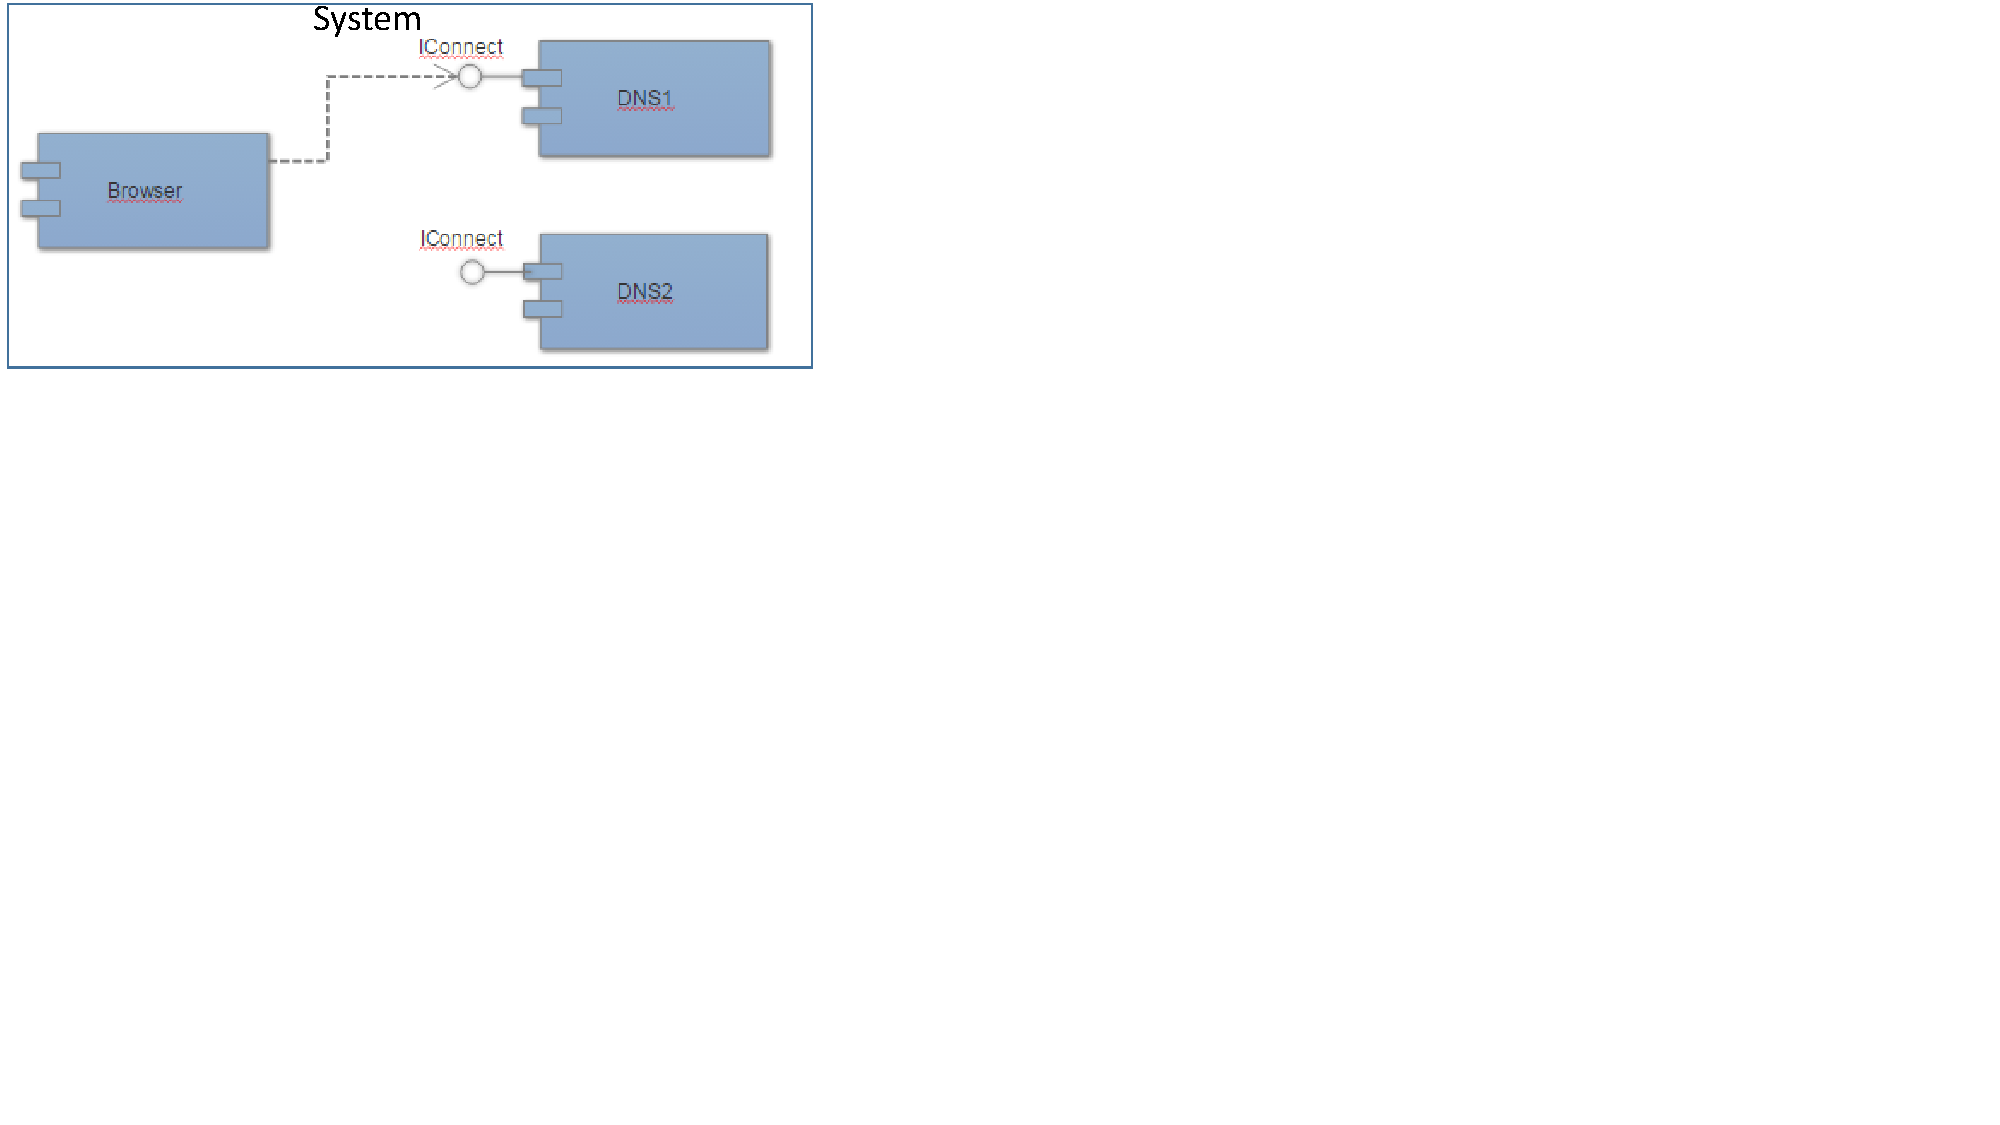
\includegraphics[clip, trim=0cm 12.4cm 19.4cm 0cm, width=\columnwidth]{figures/architectureexample.pdf}
	\caption{Component-based architecture example in CDL} 
	\label{fig:architectureexample}
\end{figure}



\begin{minipage}{0.95\columnwidth}
\lstinputlisting[language=C++, caption=Front-end code generated from the Browser in Fig. \ref{fig:architectureexample}, label=lst:front-end2,frame=f]{code/browser.cpp}
\end{minipage}

\begin{minipage}{0.95\columnwidth}
\lstinputlisting[language=C++, caption=Front-end code generated from the DNS in Fig. \ref{fig:architectureexample}, label=lst:front-end2,frame=f]{code/dns.cpp}
\end{minipage}

\begin{minipage}{0.95\columnwidth}
\lstinputlisting[language=C++, caption=Front-end code generated from the System in Fig. \ref{fig:architectureexample}, label=lst:front-end2,frame=f]{code/system.cpp}
\end{minipage}


\begin{itemize}
	\item A port can provide or require multiple interfaces/data
	
	\item For port p of component C
	
	\begin{itemize}
		\item If p provides an interface I => C must implement I or one of C's sub-com implements
		\item If p requires an interface I => invocations via p (pIConnect -> connect(), e.g.)
		\item If p provides a data signal Sig => C sends signal via p by calling p->sendSig
		\item If p uses a data signal Sig => C/C's sub-component implements ISig interface, which contains only a method sendSig(Sig\& sig);
	\end{itemize}
	
	\item Two ports p1 and p2 are matches for binding if one of the following cases:
	\begin{itemize}
		\item Assemble: All required interfaces of p1 (p2) match with all provided interfaces of p2 (p1) and all provided signals of p1 (p2) match with all required signals of p2 (p1)
		
		\item Delegation: All required interfaces of p1 (p2) match with all required interfaces of p2 (p1) and all provided signals of p1 (p2) match with all provided signals of p2 (p1)
	\end{itemize}
	
	\item Match: A match B => A = B or A inherits from B.
	
\end{itemize}

\begin{minipage}{0.95\columnwidth}
	\lstinputlisting[language=C++, caption=Multi-interface/data port front-end code, label=lst:front-end2,frame=f]{code/multiport-frontend.cpp}
\end{minipage}


\begin{minipage}{0.95\columnwidth}
\lstinputlisting[language=C++, caption=Multi-interface/data port front-end code, label=lst:front-end2,frame=f]{code/multiport-cpp.cpp}
\end{minipage}